\input{CS231a.tex}

\begin{document}

\HomeworkStudentSolutionsHeader{1}{Friday, January 29}{YOUR NAME}{YOUR EMAIL}

\section{Projective Geometry Problems [20 points]}
In this question, we will examine properties of projective transformations. We define a camera coordinate system, which is only rotated and translated from a world coordinate system.
\begin{itemize}
    \item[(a)]Prove that parallel lines in the world reference system are still parallel in the camera reference system. {\bf [4 points]}

    \item[(b)]Consider a unit square $pqrs$ in the world reference system where $p, q, r, $ and $s$ are points. Will the same square in the camera reference system always have unit area? Prove or provide a counterexample. {\bf [4 points]}

    \item[(c)]Now let's consider affine transformations, which are any transformations that preserve parallelism. Affine transformations include not only rotations and translations, but also scaling and shearing. Given some vector $p$, an affine transformation is defined as \[A(p) = Mp + b\] where $M$ is an invertible matrix. Prove that under any affine transformation, the ratio of parallel line segments is invariant, but the ratio of non-parallel line segments is not invariant. {\bf [6 points]}

    \item[(d)]You have explored whether these three properties hold for affine transformations. Do these properties hold under any projective transformation? Justify briefly in one or two sentences (no proof needed). {\bf [6 points]}
\end{itemize}


\section{Affine Camera Calibration (35 points)}

In this question, we will perform affine camera calibration using two different images of a calibration grid.  First, you will find correspondences between the corners of the calibration grids and the 3D scene coordinates.  Next, you will solve for the camera parameters.

It was shown in class that a perspective camera can be modeled using a 3 $\times$ 4 matrix:
\begin{equation}
\left [
\begin{matrix}
x \\
y \\
w
\end{matrix}
\right ] = \left [
\begin{matrix}
p_{11} & p_{12} & p_{13} & p_{14} \\
p_{21} & p_{22} & p_{23} & p_{24} \\
p_{31} & p_{32} & p_{33} & p_{34}
\end{matrix}
\right ] \left [
\begin{matrix}
X \\
Y \\
Z \\
1
\end{matrix}
\right ]
\end{equation}
which means that the image at point $(X, Y , Z )$ in the scene has pixel coordinates $(x/w, y/w)$. The 3 $\times$ 4 matrix can be factorized into intrinsic and extrinsic parameters.

An \emph{affine} camera is a special case of this model in which rays joining a point in the scene to its projection on the image plane are parallel. Examples of affine cameras include orthographic projection and weakly perspective projection. An affine camera can be modeled as:

\begin{equation}
\left [
\begin{matrix}
x \\
y \\
1
\end{matrix}
\right ] = \left [
\begin{matrix}
p_{11} & p_{12} & p_{13} & p_{14} \\
p_{21} & p_{22} & p_{23} & p_{24} \\
0 & 0 & 0 & 1
\end{matrix}
\right ] \left [
\begin{matrix}
X \\
Y \\
Z \\
1
\end{matrix}
\right ]
\end{equation}
which gives the relation between a scene point $(X, Y , Z )$ and its image $(x, y)$. The difference is that the bottom row of the matrix is $[\ 0 \ \ 0 \ \ 0 \ \ 1\ ]$, so there are fewer parameters we need to calibrate. More importantly, there is no division required (the homogeneous coordinate is 1) which means this is a \emph{linear model}. This makes the affine model much simpler to work with mathematically - at the cost of losing some accuracy. The affine model is used as an approximation of the perspective model when the loss of accuracy can be tolerated, or to reduce the number of parameters being modeled.
\begin{figure}[ht!]
  \centering
  \subfloat[Image formation in an affine camera.  Points are projected via parallel rays onto the image plane]{\includegraphics[width=5in]{cameraSetup.png}} \\
  \subfloat[Image of calibration grid at Z=0]{\includegraphics[width=2.3in]{fig1imgAlabel.jpg}} \
  \subfloat[Image of calibration grid at Z=150]{\includegraphics[width=2.3in]{fig1imgblabel.jpg}}
  \caption{Affine camera: image formation and calibration images.}
  \label{fig:aff}
\end{figure}
Calibration of an affine camera involves estimating the 8 unknown entries of the matrix in Eq. 2 (This matrix can also be factorized into intrinsics and extrinsics, but that is outside the scope of this homework). Factorization is accomplished by having the camera observe a calibration pattern with easy-to-detect corners.
\\
\\
\textbf{Scene Coordinate System}
\\
\\
The calibration pattern used is shown in Figure 1, which has a $6 \times 6$ grid of squares. Each square is $50mm \times 50mm$. The separation between adjacent squares is $30mm$, so the entire grid is $450mm \times 450mm$. For calibration, images of the pattern at two different positions were captured. These images are shown in Fig. 1 and can be downloaded from the course website. For the second image, the calibration pattern has been moved back (along its normal) from the rest position by $150mm$.

We will choose the origin of our 3D coordinate system to be the top left corner of the calibration pattern
in the rest position. The $X$-axis runs left to right parallel to the rows of squares. The $Y$-axis runs top to
bottom parallel to the columns of squares. We will work in units of millimeters. All the square corners from
the first position corresponds to $Z = 0$. The second position of the calibration grid corresponds to $Z =150$.  The top left corner in the first image has 3D scene
coordinates $(0,0,0)$ and the bottom right corner in the second image has 3D scene coordinates $(450,450,150)$. This scene coordinate system is labeled in Fig. 1.

\begin{itemize}
  \item[(a)] Given correspondences for the calibrating grid, solve for the camera parameters using Eq. 2. Note that each measurement $(x_i , y_i )  \leftrightarrow (X_i , Y_i , Z_i )$ yields two linear equations for the 8 unknown camera parameters. Given $N$ corner measurements, we have $2N$ equations and 8 unknowns. Using the given corner correspondences as inputs, complete the method \texttt{compute\_camera\_matrix()}. You will construct a linear system of equations and solve for the camera parameters to minimize the least-squares error. After doing so, you will return the $3\times4$ affine camera matrix composed of these computed camera parameters. In your written report, submit your code as well as the camera matrix that you compute. {\bf [15 points]}

  \item[(b)] After finding the calibrated camera matrix, you will compute the RMS error between the given $N$ image corner coordinates and $N$ corresponding calculated corner locations in \texttt{rms\_error()}.  Recall that \[\mathrm{RMS}_\mathrm{total}=\sqrt{ \sum ((x-x')^2 + (y-y')^2)/N}\]
  Please submit your code and the RMS error for the camera matrix that you found in part (a). {\bf [15 points]}

	\item[(c)] Could you calibrate the matrix with only one checkerboard image? Explain briefly in one or two sentences. {\bf [5 points]}


\end{itemize}


\section{Single View Geometry (45 points)}
\begin{figure}[h!]
	\centering
	\subfloat[Image 1 (1.jpg) with marked pixels]{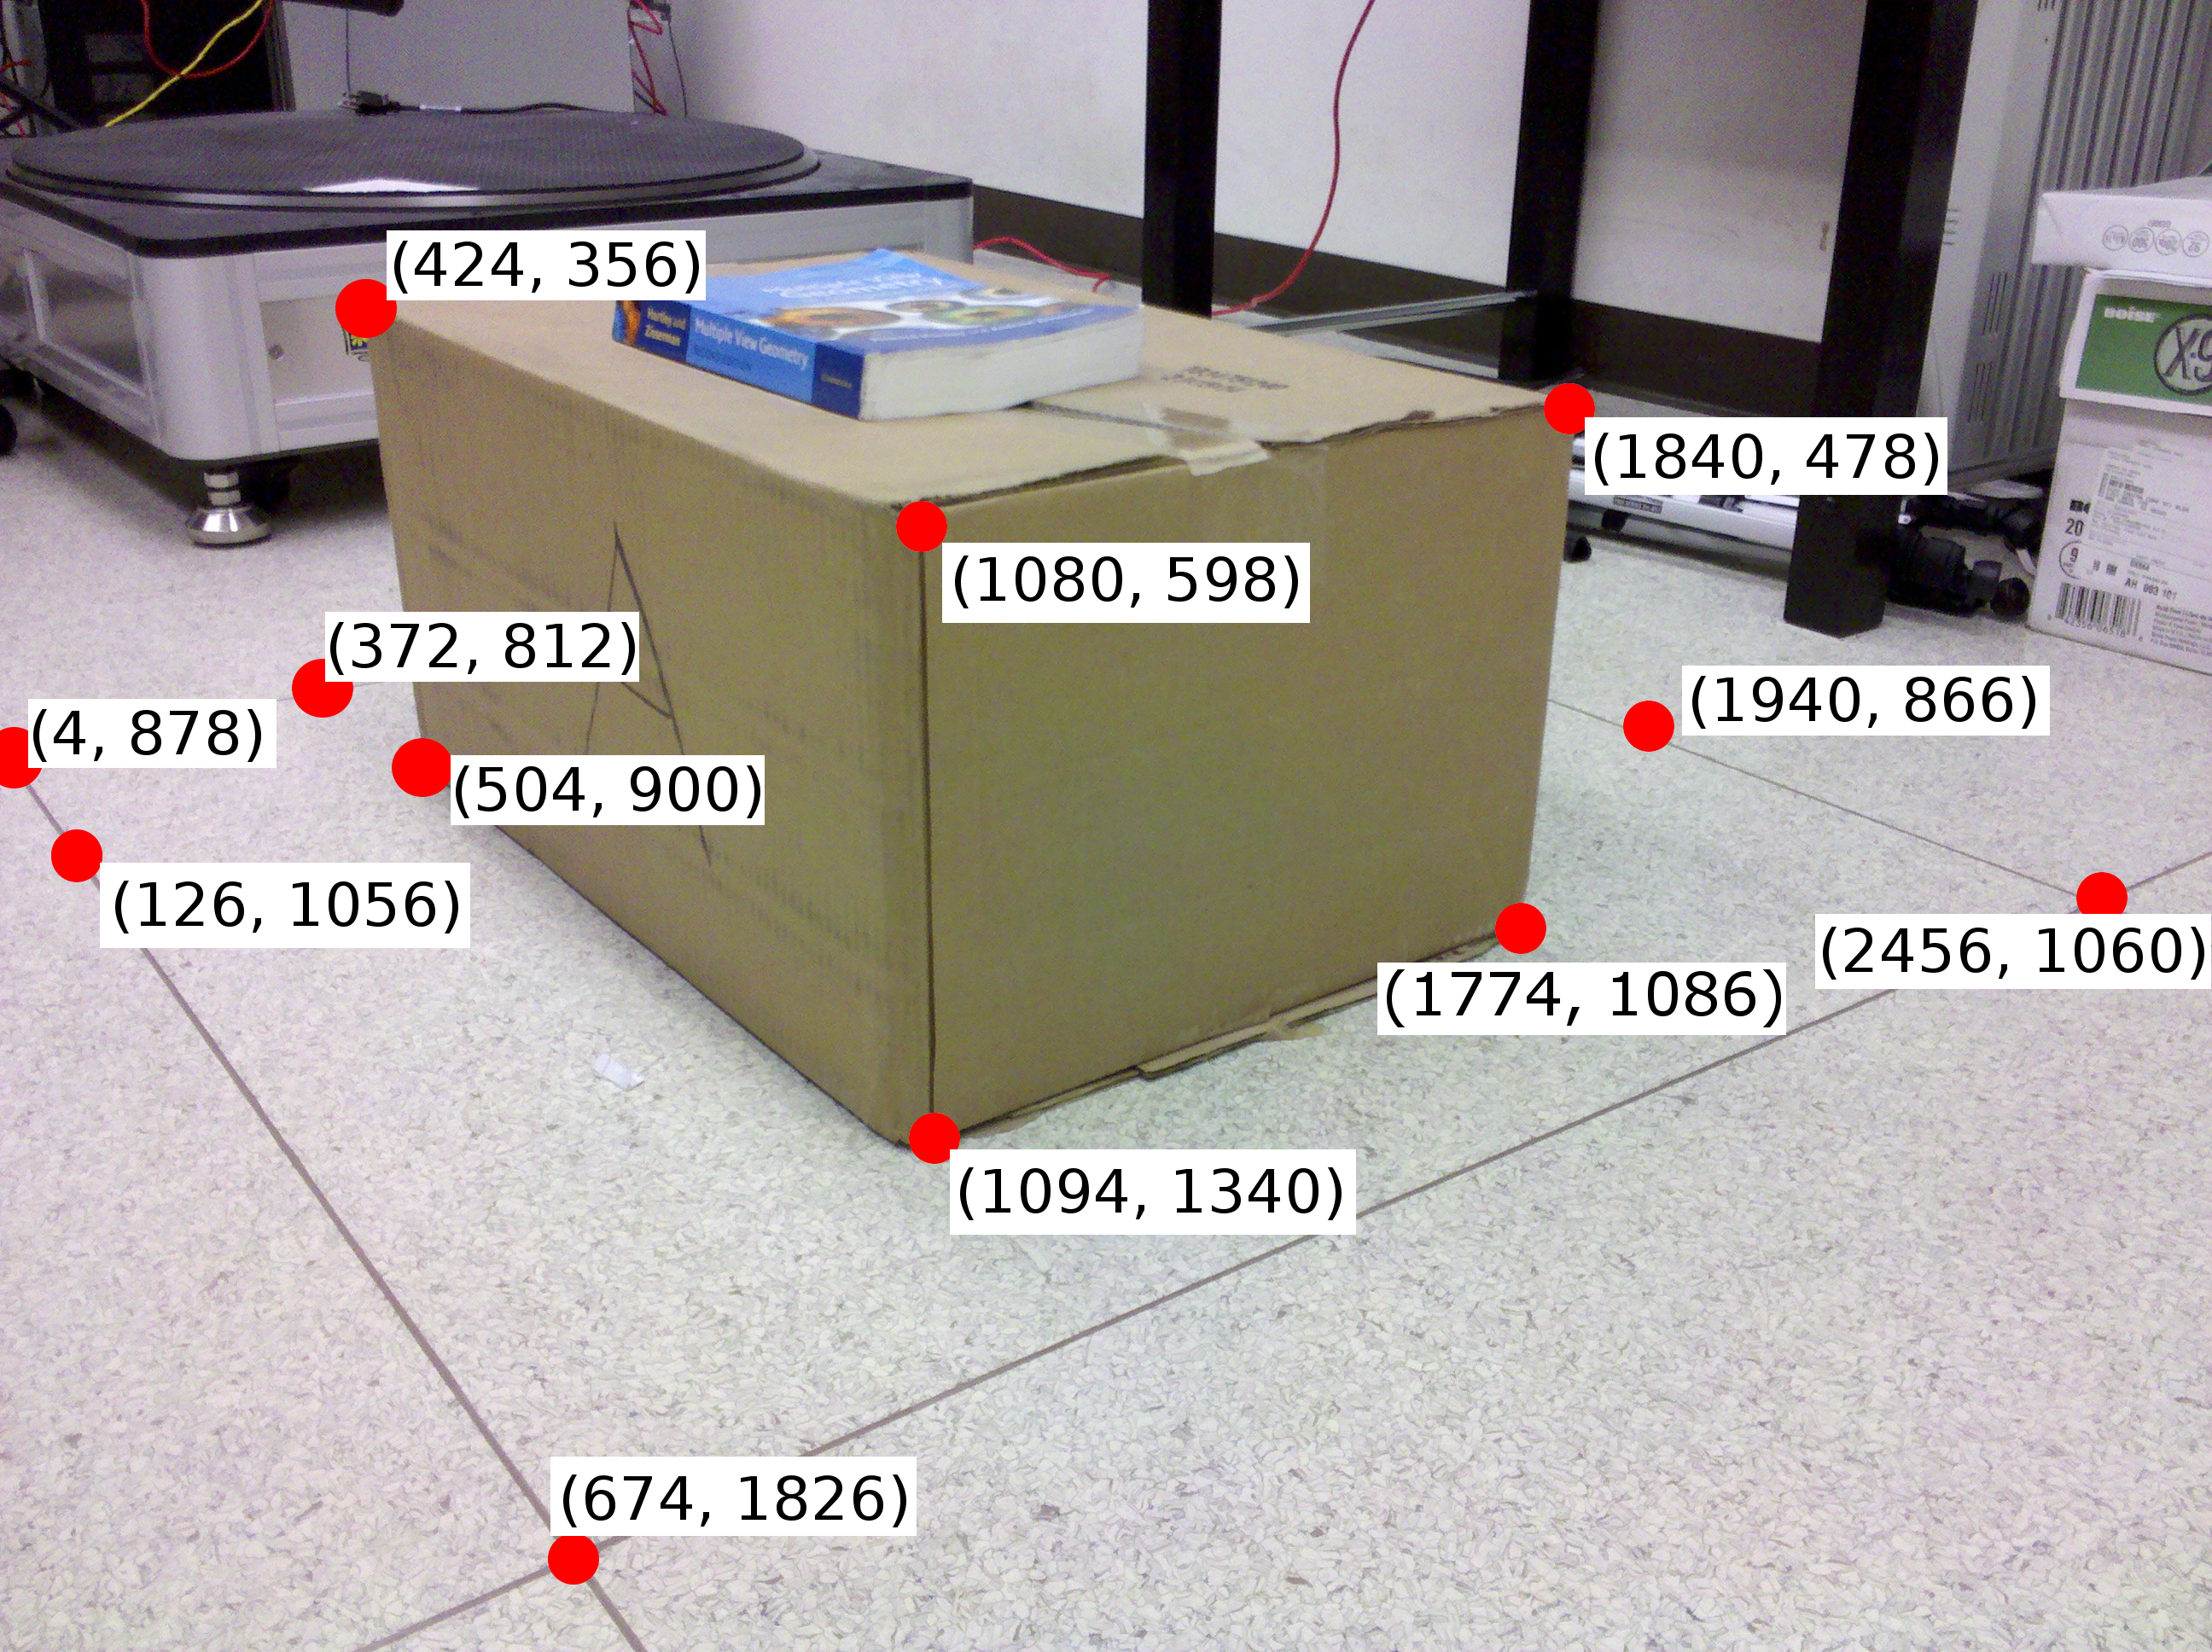
\includegraphics[width=2.5in]{1_with_points.png}} \
	\subfloat[Image 2 (2.jpg) with marked pixels]{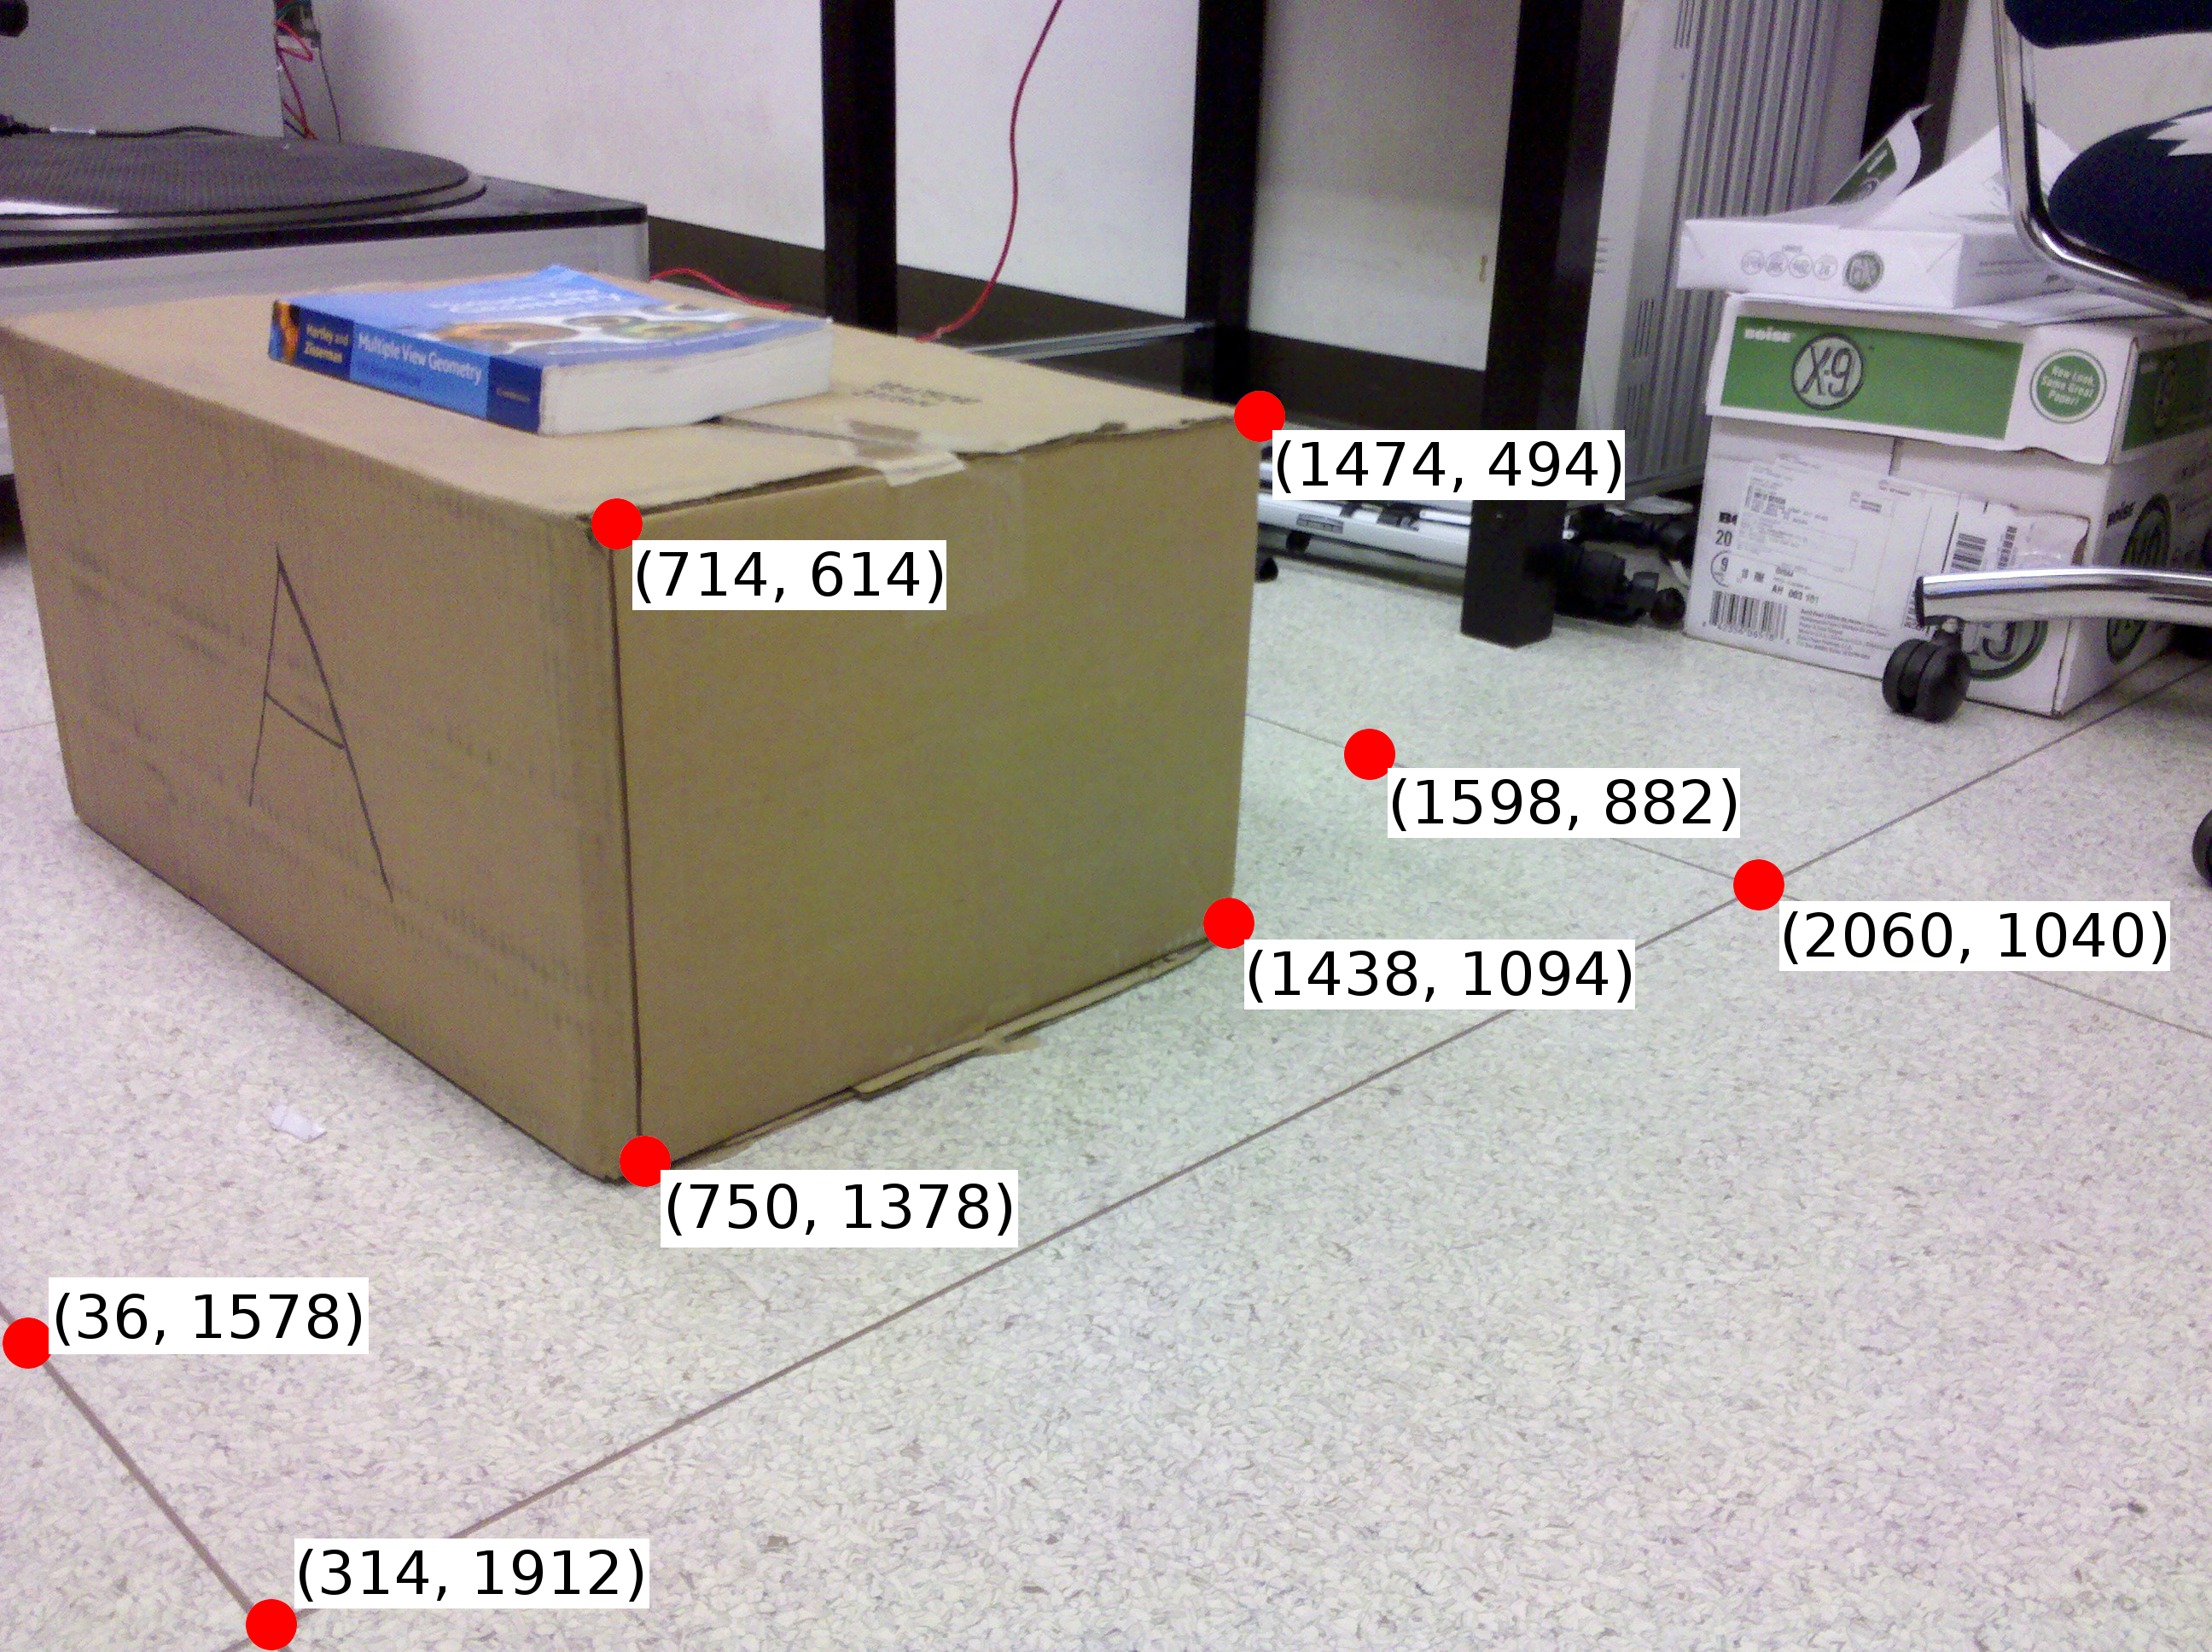
\includegraphics[width=2.5in]{2_with_points.png}}
	\label{fig:singleView}
  \caption{Marked pixels in images taken from different viewpoints.}
\end{figure}

In this question, we will estimate camera parameters from a single view and leverage the projective nature of cameras to find both the camera center and focal length from vanishing points present in the scene above.

\begin{itemize}
\item[(a)]  In Figure 2, we have identified a set of pixels to compute vanishing points in each image. Please complete \texttt{compute\_vanishing\_point()}, which takes in these two pairs of points on parallel lines to find the vanishing point. You can assume that the camera has zero skew and square pixels, with no distortion. {\bf [5 points]}

\item[(b)] Using three vanishing points, we can compute the intrinsic camera matrix used to take the image. Do so in \texttt{compute\_K\_from\_vanishing\_points()}. {\bf [10 points]}

\item[(c)] Is it possible to compute the camera intrinsic matrix for any set of vanishing points? Similarly, is three vanishing points the minimum required to compute the intrinsic camera matrix? Justify your answer. {\bf [5 points]}

\item[(d)] The method used to obtain vanishing points is approximate and prone to noise. Discuss approaches to refine this process. {\bf [5 points]}

\item[(e)] This process gives the camera internal matrix under the specified constraints. For the remainder of the computations, use the following internal camera matrix:

 \[
  K = \left [
  \begin{matrix}
  2448 & 0 & 1253 \\
  0 & 2438 & 986 \\
  0 & 0 & 1
  \end{matrix}
  \right ]
    \]
 Identify a sufficient set of vanishing lines on the ground plane and the plane on which the letter A exists, written on the side of the cardboard box, (plane-A). Use these vanishing lines to verify numerically that the ground plane is orthogonal to the plane-A. Fill out the method \texttt{compute\_angle\_between\_planes()} and submit your code and the computed angle. {\bf [10 points]}

\item[(f)] Assume the camera rotates but no translation takes place. Assume the internal camera parameters remain unchanged. An Image 2 of the same scene is taken. Use vanishing points to estimate the rotation matrix between when the camera took Image 1 and Image 2. Fill out the method \texttt{compute\_rotation\_matrix\_between\_cameras()} and submit your code and your results. {\bf [10 points]}
\end{itemize}


\end{document}

